\chapter{Resultados experimentales}

\section{Comparación de parámetros $P$ y $N$}
Como se explicó en el capítulo anterior, el algoritmo desarrollado depende de dos parámetros: $G$, o la frecuencia con la que realizamos la fase constructiva; y $N$, el número máximo de vuelos que puede contener la cola de vuelos extras.\\
Tras realizar varias pruebas, hemos podido comprobar que los mejores resultados se obtienen con un parámetro $N$ pequeño y $G$ grande:
\begin{itemize}
	\item Un \textbf{\textit{N} pequeño} implica realizar la fase constructiva con mucha frecuencia. Esto hace que cada pocas iteraciones busquemos un intento de mejora, y por tanto en caso de no conseguir mejorar la solución actual descartaremos la cola de vuelos extras con mucha rapidez.\\
	Un $N$ pequeño también aporta más desviación a los resultados, ya que al descartar colas con mucha facilidad, hace que el problema se reinicie con más frecuencia, y por tanto tenga más aleatoriedad. 
	
	\item Un \textbf{\textit{G} grande} implica que se de más peso a las buenas soluciones que se localizaron en la cola anterior. Por tanto al tener una cola de vuelos extras de gran tamaño, permite que las buenas soluciones tengan una probabilidad mucho mayor que salir antes.
\end{itemize} 

A continuación se muestran los resultados que hemos obtenido aplicando distintos parámetros a los casos de prueba de los que disponíamos:

\begin{figure}[H]
	\begin{center}
		\centering
		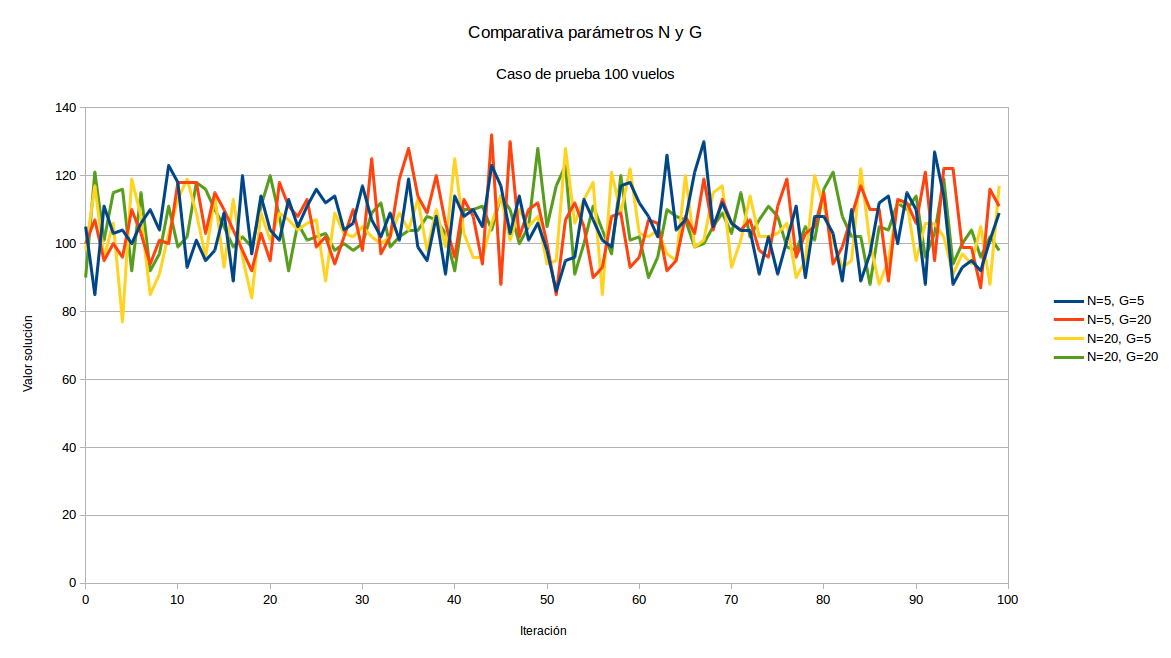
\includegraphics[width=1\textwidth]{./imagenes/heuristico/comparativa_parametros_100_vuelos.png}
		\caption{Comparativa de parámetros G y N}
		\label{fig: Comparativa de parámetros G y N}
	\end{center}
\end{figure}


\begin{table}[htbp]
	\centering
	\caption{Comparativa de parámetros $G$ y $N$.}
	\label{fig: comparativa de parámetros $G$ y $N$.}
\begin{tabular}{|c|c|c|c|}
	\hline
	& \textbf{Problema 1
		100 vuelos} & \textbf{Problema 2
		100 vuelos} & \textbf{Problema 3
		100 vuelos} \\ \hline
	\textbf{N=2, G=10} & \% éxito: 64 & \% éxito: 94 &  \\ \hline
	\textbf{N=2, G=30} & \% éxito: 65 & \% éxito: 95 &  \\ \hline
	\textbf{N=2, G=50} &  &  &  \\ \hline
	\textbf{N=5, G=10} &  &  &  \\ \hline
	\textbf{N=5, G=30} &  &  &  \\ \hline
	\textbf{N=5, G=50} &  &  &  \\ \hline
	\textbf{N=10, G=10} &  &  &  \\ \hline
	\textbf{N=10, G=30} &  &  &  \\ \hline
	\textbf{N=10, G=50} &  &  &  \\ \hline
\end{tabular}
	
\end{table}

\section{Evolución de la función objetivo}
A continuación se muestra la evolución de la función objetivo para diferentes parámetros de $N$ y $G$
\section{Resultado obtenidos}


